\section{Results}\label{section:results}

\subsection{\pt-differential cross section of heavy-flavour decay electrons in pp and \pPb collisions}
The $p_{\rm{T}}$-differential production cross section of electrons from semileptonic heavy-flavour hadron decays at midrapidity
in pp collisions at $\sqrt{s} = 13$ TeV measured in the transverse momentum region $0.2 < p_{\rm{T}} < 35$ GeV$/c$ is shown in Fig.~\ref{Fig:ppHFESpectra} (left). While the statistical errors are presented as vertical lines, the total systematic uncertainties are given by the rectangular box. The figure  presents the comparison of the cross section measured using two different data sets collected with different magnetic fields in the overlapping $p_{\rm{T}}$ interval of 0.5--4.0~GeV$/c$, and the comparison of the measurement performed using TPC--TOF and TPC--EMCal detectors in the interval of 3.0--4.0 GeV$/c$. The bottom panel of the Fig.~\ref{Fig:ppHFESpectra} presents the ratio of the cross-sections, obtained using different data sets and different detectors, in the overlapping $p_{\rm{T}}$ intervals, which shows that they are consistent with each other within the statistical and systematic uncertainties. 
%obtained using different data sets and different detectors. The cross sections in these $p_{\rm{T}}$ intervals are consistent with each other within the statistical and systematic uncertainties. 
The cross sections obtained with MB triggered sample (using TPC--EMCal) and EMCal triggered samples, EG2 and EG1, are also compared in the interval 6.0--10.0 GeV$/c$ and 12.0--18.0 GeV$/c$, respectively, the ratio of which are presented in the bottom panel of the figure, and are consistent within the uncertainties.  

The $p_{\rm{T}}$-differential cross section measurement is compared with the Fixed-Order-Next-to-Leading-Log (FONLL)~\cite{Cacciari:1998it} pQCD calculation, as shown in the right panel of Fig.~\ref{Fig:ppHFESpectra}. The uncertainties of the FONLL calculations reflect different choices for the charm and beauty quark masses, and for the factorisation and renormalization scales as well as the uncertainty on the set of parton distribution functions (PDF) used in the pQCD calculations (CTEQ6.6~\cite{Nadolsky:2008zw}). The FONLL calculations describe the measurements within the statistical and systematic uncertainties and the data is found be close to the upper edge of the theoretical prediction, which can be better seen in the bottom panel of the figure, which presents the ratio of the data points to the FONLL calculations. 
%up to $p_{\rm{T}} < 5$ GeV$/c$, 
Similar observations were done in pp collisions at $\sqrt{s} = 2.76,$ $5.02$ and $7$ TeV~\cite{Abelev:2014gla, Acharya:2018upq, Acharya:2019mom, Abelev:2012xe}. Electrons from heavy-flavour hadron decays are dominated by semi-leptonic decays of beauty hadrons for \pt~$>5$ ~GeV/$c$~\cite{Abelev:2012sca, Abelev:2014hla}, hence the cross section measured up to 36 GeV/$c$ can provide important information to beauty hadron production. 
%Measurements of electrons from heavy-flavour hadron decays at high \pt provide important information to beauty hadron production, which is the dominant contribution to the cross section for \pt $>$ 5 GeV/$c$.   %The dominant contribution from electrons from semileptonic beauty hadron decays is expected at higher $p_{\rm {T}}$ and therefore, the measurement is extended to high $p_{\rm {T}}$.
%, while at higher $p_{\rm{T}}$, the measurement is close to the mean value of the FONLL prediction.

\begin{figure}[!ht]
\centering

%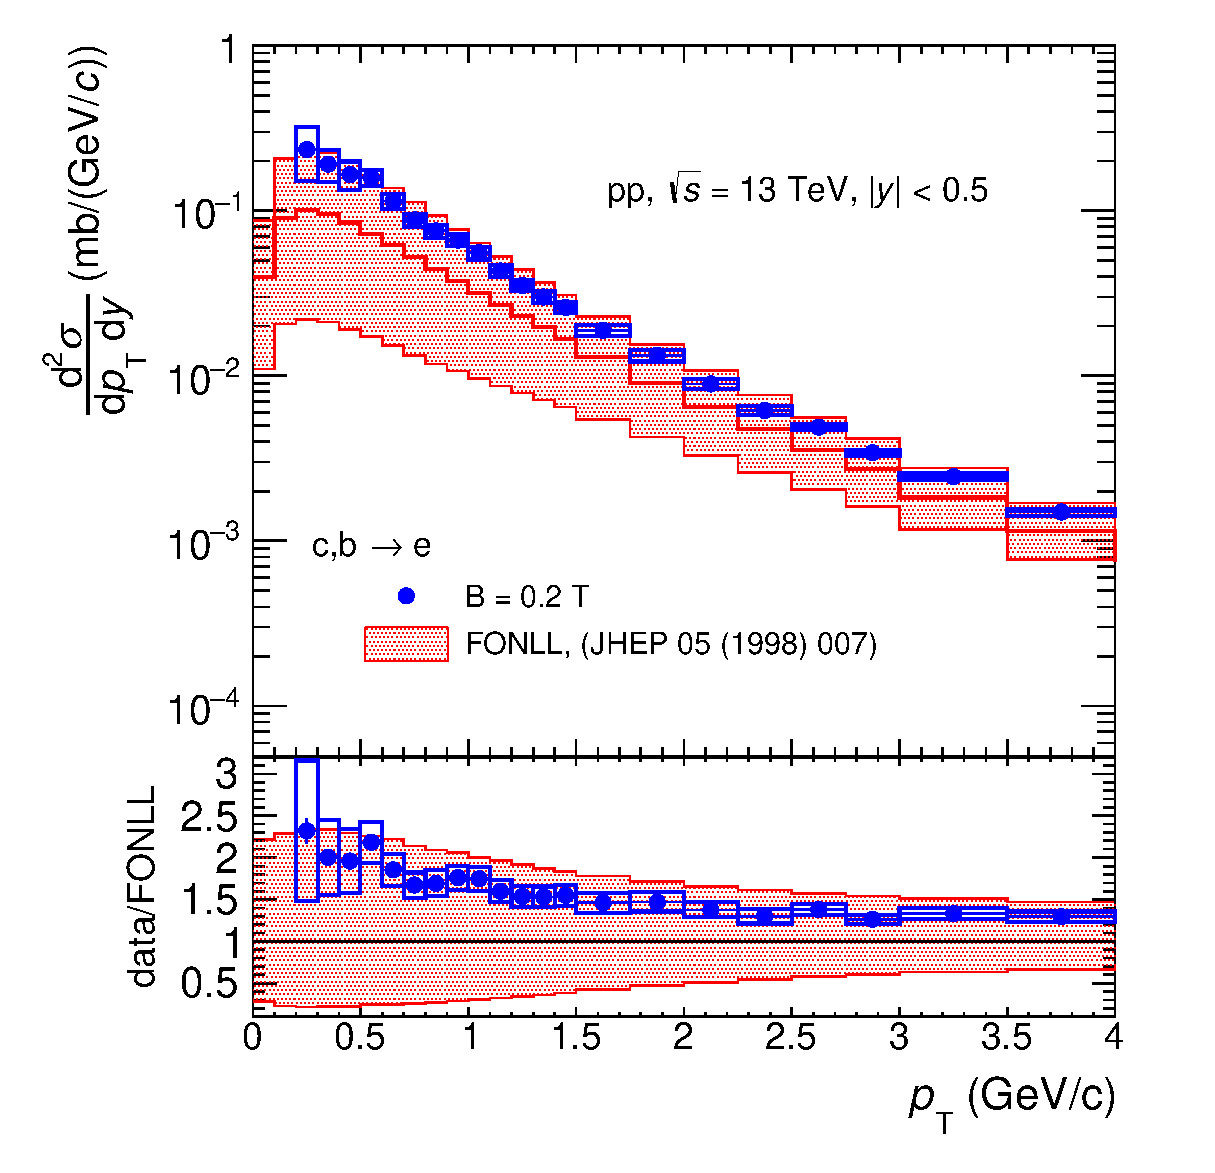
\includegraphics[scale = 0.3]{figurehttp://arxiv.org/abs/hep-ph/9803400s/Results/HFE_pp_LowB/HFE_comparison_05_lowB_with_FONLL_WSyst_Oct27_2020_UpEdgeKe3_CentralPointsHFE.eps}
\includegraphics[width=0.48\linewidth]{figures/Results/HFE_ppNormalB/HFE_Comparison_1.pdf}
\includegraphics[width=0.48\linewidth]{figures/Results/HFE_ppNormalB/Data_FONLL_HFE_1.pdf}
\caption{Left: In the upper panel, $p_{\rm T}$-differential cross section of electrons from heavy-flavour hadrons decays in pp collisions at $\sqrt{s} =$ 13 TeV measured at midrapidity with different detectors and datasets. In the bottom panel, ratios of the different measurements in the overlapping pt intervals. Right: In the upper panel, the $p_{\rm{T}}$ differential cross section is compared with FONLL predictions~\cite{Cacciari:1998it} and its ratio with respect to FONLL central value is shown in the bottom panel. Vertical bars and boxes denote statistical and systematical uncertainties, respectively.}        
\label{Fig:ppHFESpectra}
\end{figure}

\begin{figure}[!ht]
\centering
\includegraphics[width=0.5\linewidth]{figures/Results/HFE_pPb/HFE_InvariantCrossSection_pPb.pdf}
\caption{The $p_{\rm{T}}$ differential cross section of electrons from heavy-flavour hadron decays in \pPb collisions at \sqrtsNN = 8.16 TeV with TPC--TOF (blue data points) and TPC--EMCal (red data points).}        
\label{Fig:pPbHFESpectra}
\end{figure}

% Figure~\ref{Fig:ppHFESpectra} depicts the comparison of the cross section measured using using TPC--TOF (low and normal B) and TPC--EMCal detectors in the interval of xx-yy GeV$/c$. The cross sections are consistent with each other within the statistical and systematic uncertainties. The cross sections obtained with MB triggered sample (using TPC--EMCal) and EMCal triggered samples, EG2 and EG1, are also compared in the interval xx-yy GeV$/c$ and xx-yy GeV$/c$, respectively and are consistent within the uncertainties. 

 The $p_{\rm{T}}$-differential production cross section of electrons from semileptonic heavy-flavour hadron decays at midrapidity in \pPb collisions at $\sqrt{s_{\rm{NN}}} = 8.16$ TeV measured in the transverse momentum region $0.5 < p_{\rm{T}} < 26$~GeV$/c$ is shown in Fig.~\ref{Fig:pPbHFESpectra}. The statistical errors are presented as horizontal lines, the total systematic uncertainties are represented by the rectangular box. The Fig.~\ref{Fig:pPbHFESpectra} also presents the comparison of the cross section measured using using TPC--TOF and TPC--EMCal detectors in the interval of 3.0--4.0 GeV$/c$. The ratio of the cross-section measured using different detectors in the overlapping \pt range is presented in the bottom panel of the figure. The cross sections are consistent with each other within the statistical and systematic uncertainties. The cross sections obtained with MB triggered sample (using TPC--EMCal) and EMCal triggered sample, EG2 and EG1, are also compared in the interval  6.0--10.0 GeV$/c$ and 10.0--14.0 GeV$/c$, respectively, the ratio of which are presented in the bottom panel of the figure, and are consistent within the uncertainties. 

The nuclear modification factor, $R_{\rm{pPb}}$, requires a reference cross section for pp collisions at the same centre-of-mass energy. This was obtained by a $\sqrt{s}$-scaling procedure using pQCD calculations. The $p_{\rm{T}}$-dependent scaling factor was obtained by calculating the ratio of the production cross sections of electrons from heavy-flavour hadron decays from fixed order with next-to-leading-log (FONLL) calculations~\cite{Cacciari:1998it,Cacciari:2001td, Cacciari:2012ny} at $\sqrt{s}=13$ TeV to $\sqrt{s}=8.16$ TeV. The systematic uncertainty on the pp reference includes the systematic uncertainties on the measured cross section at $\sqrt{s}=13$ TeV, which is described above, and the $p_{\rm{T}}$-dependent scaling factor. The uncertainty on the scale factor ranges between 11--1\% and includes the uncertainties on the Parton Distribution Functions, quark masses, and factorisation and renormalization scales, as described in~\cite{Averbeck:2011ga}. The two contributions are added in quadrature leading to a total systematic of  $15–5\%$, depending on $p_{\rm{T}}$. In addition, a global normalization systematic uncertainty of 5\% from the pp analysis at $\sqrt{s}=13$ TeV was also considered. Figure ~\ref{Fig:HFESpectraComparison} shows the comparison of the $\sqrt{s}$-scaled  production cross sections of electron from heavy-flavour hadron decays in pp collisions at \sqrts = 13 TeV using aforementioned procedure with the production cross sections of electron from heavy-flavour hadron decays in \pPb collisions at \sqrtsNN = 8.16 TeV.

\subsection{Nuclear modification factor of electrons from heavy-flavour hadron decays in \pPb collisions}
The nuclear modification factor, $R_{\rm{pPb}}$, of electrons from heavy-flavour hadron decays as a function of transverse momentum at $\sqrt{s_{\rm{NN}}} = 8.16$ TeV is presented in Fig.~\ref{Fig:RpPb}. The statistical and systematic uncertainties of the spectra in p–Pb and pp collisions were propagated as uncorrelated. The normalization uncertainties are shown as a solid box at $R_{\rm{pPb}} = 1$. The $R_{\rm{pPb}}$ is consistent with unity within statistical and systematic uncertainties over the whole $p_{\rm{T}}$ range of the
measurement. Thus, the measurements are consistent with no modification over the measured $p_{\rm{T}}$ range. The sample of electrons from heavy-flavor hadron decays is dominated by beauty-hadron decays for $p_{\rm{T}} > 5$ GeV$/c$~\cite{Abelev:2012sca, Abelev:2014hla}. The $R_{\rm{pPb}}$ of unity indicates that the beauty production is not modified in \pPb collisions within the kinematic range of this measurement, which is also consistent with the measurement of $R_{\rm{pPb}}$ of beauty-decay electrons upto $p_{\rm{T}} = 8$ GeV$/c$ at $\sqrt{s_{\rm{NN}}} = 5.02$ TeV~\cite{Adam:2016wyz}. 

\begin{figure}[!ht]
\centering
\includegraphics[width=0.5\linewidth]{figures/Results/HFE_pPb/ppScaledReference.pdf}
\caption{The $p_{\rm{T}}$ differential cross section of electrons from heavy-flavour hadron decays in \pPb collisions at \sqrtsNN = 8.16 TeV compared with pp at \sqrts = 13 TeV scaled reference.}        
\label{Fig:HFESpectraComparison}
\end{figure}

\begin{figure}[!ht]
      \begin{center}
      \includegraphics[width=0.48\linewidth]{figures/Results/HFE_pPb/RpPb_8TeV.pdf}
      \includegraphics[width=0.48\linewidth]{figures/Results/HFE_pPb/RpPb_8TeV_ComparedWith5TeV.pdf}
      \end{center}
\caption{The nuclear modification factor ($R_{\rm{pPb}}$) of electrons from heavy-flavour hadron decays in \pPb collisions at \sqrtsNN = 8.16 TeV (left) and the $R_{\rm{pPb}}$ at \sqrtsNN = 8.16 TeV is compared with that at \sqrtsNN = 5.02 TeV and theoretical models at \sqrtsNN = 5.02 TeV (right).}    
\label{Fig:RpPb}
\end{figure}

\subsection[Self-normalized yield of electrons from heavy-flavour decays vs. normalized multiplicity]{Self-normalized yield of electrons from heavy-flavour decays vs. normalized multiplicity in pp and \pPb collisions}
The yield of electrons from heavy-flavour hadron decays was measured as described above in multiplicity intervals, and its ratio in a given multiplicity interval relative to the minimum bias yield is computed. The normalized yield of electrons from heavy-flavour decays, $\dndeta/\left<\dndeta\right>$, as a function of normalized charged-particle pseudorapidity density at midrapidity, $\dnchdeta/\left<\dnchdeta\right>$, is presented in Fig.~\ref{Fig:SelfnormalizedYield} in pp collisions at $\sqrt{s} =$ 13 TeV and in \pPb collisions at $\sqrt{s_{NN}}$ $=$ 8.16 TeV.  The results are normalized to INEL$>0$ event class. The measurements were performed in five $p_{\rm T}$ intervals from 0.5--30 GeV$/c$ for pp collisions and from 0.5--26 GeV$/c$ for \pPb collisions. The dashed line shown in the figure is a linear function with a slope of unity. The normalized yield allows us to examine events with a multiplicity more than 6 times (4 times) larger than the average multiplicity in pp (\pPb) collisions. In both pp and \pPb collisions, the normalized heavy-flavour decay electron yield grows faster than linear with the normalized multiplicity. This measurement is similar to the trend observed for inclusive charged-particle production~\cite{Acharya:2019mzb}, strange hadrons~\cite{Acharya:2019kyh}, D-mesons~\cite{Adam:2015ota,Adam:2016mkz},  J/$\psi$~\cite{Acharya:2020pit,Abelev:2012rz,Acharya:2020giw} and $\Upsilon$ mesons~\cite{Chatrchyan:2013nza}.
The bottom panel of Fig.~\ref{Fig:SelfnormalizedYield} shows the double ratio of the normalized heavy-flavour decay electron yield to the normalized multiplicity. It can be observed that for both pp and \pPb collisions the double ratio increases with multiplicity. In \pPb collisions, the increase is stronger for events with small multiplicity and slightly weaker increase at high multiplicity, and no dependence on \pt is observed. In pp collisions, while a strong increase is observed at low multiplicities for all \pt, the increase is weaker for low \pt electrons and a strong increase is seen for high \pt particles at higher multiplicities. The double ratio was fit with a linear function, as shown in Fig.~\ref{Fig:SNY_Ratio_pp} (right), and found to reasonable describe the data for all \pt bins. This indicates that in the measured \pt range the yield increases approx. with the square of the multiplicity with a coefficient which increases with \pt.

The measurement in pp collisions in intervals of $\pt$ shows that high $\pt$ heavy-flavour decay electron yield increases faster than the charged-particle multiplicity, while the
increase is smaller when we consider lower-$\pt$ particles. The yield increase is approximately a factor of 9 for the lowest measured $\pt$ ($0.5 < \pt < 1.5$ GeV$/c$) and a factor of 32 for the highest measured $\pt$ ($20 < \pt < 35$ GeV$/c$) for multiplicities of 6 times the average multiplicity. In the left panel of Fig.~\ref{Fig:SNY_Ratio_pp} the ratios of the average of the heavy-flavour decay electron relative yields in various \pt
intervals with respect to the $6 < \pt < 12$ GeV$/c$ interval values is shown. The yield of lower $\pt$ electrons is higher in low  multiplicity events, while it reduces in higher multiplicity events. Electrons at higher $\pt$ has an opposite trend, where the yield is lower in low  multiplicity events and increases at higher multiplicity. It should be noted that the contribution of heavy-flavour decay electrons from beauty hadron decays increases with $\pt$ and dominates over charm hadron decays for $\pt > 5-6$ GeV$/c$.  The observed $\pt$ dependence could be attributed to several effects - the momentum dependence of jet fragmentation affecting the measured multiplicity at midrapidity, and the momentum dependence of the fraction of electrons from charm and beauty hadron decays. 


\begin{figure}[!ht]
\includegraphics[width=0.46\linewidth]{figures/Results/HFE_ppNormalB/SNY_diagonal.pdf}
\hfil
\includegraphics[width=0.46\linewidth]{figures/Results/HFE_pPb/HFESelfNormalieYieldFullpT.pdf}
\caption{Self-normalized yield of electrons from heavy-flavour decays as a function of normalized charged-particle pseudorapidity density at midrapidity computed in \pp collisions at \sqrts = 13 TeV (left) and in \pPb collisions at \sqrtsNN = 8.16 TeV (right) in different \pt intervals.}
\label{Fig:SelfnormalizedYield}
\end{figure}

\begin{figure}[!h]
%\centering
%\includegraphics[width=0.6\linewidth]{figures/Results/HFE_ppNormalB/SNY_diagonal.pdf}
\includegraphics[width=0.48\linewidth]{figures/Results/HFE_ppNormalB/SNY_Pt_Ratio_0.pdf}
\includegraphics[width=0.48\linewidth]{figures/Results/HFE_ppNormalB/SNY_Fit_Diagonal_Linear.pdf}
\caption{ Ratio of the  normalized yield
in different \pt intervals with respect to that of the $6 < \pt < 12~{\rm GeV}/c$ interval (left) and double ratio of the normalized yield of heavy-flavour decay electrons to the normalized multiplicity in pp collisions at $\sqrts=13$ TeV (right) in three \pt ranges.}
\label{Fig:SNY_Ratio_pp}
\end{figure}

\begin{figure}[!h]
\centering
\includegraphics[width=0.5\linewidth]{figures/Results/HFE_ppNormalB/SNY_PYTHIA_0.pdf}
%\includegraphics[width=0.5\linewidth]{figures/Results/HFE_ppNormalB/SNY_PYTHIA_1.pdf}
\caption{Comparison of self-normalized yield of electrons from heavy-flavour decays computed in \pp collisions at \sqrts = 13 TeV for different \pt intervals with PYTHIA 8.2 calculations.}
     \label{Fig:SelfnormalizedYield_pp_PYTHIA}
\end{figure}

\begin{figure}[!h]
\centering
\includegraphics[width=0.45\linewidth]{figures/Results/HFE_ppNormalB/SNY_JPsi_PYTHIA_0.pdf}
\includegraphics[width=0.45\linewidth]{figures/Results/HFE_ppNormalB/SNY_ChargedParticles_High_6_10.pdf}
\includegraphics[width=0.45\linewidth]{figures/Results/HFE_ppNormalB/SNY_Dmeson_0.pdf}
\caption{Comparison of self-normalized yield of electrons from heavy-flavour decays computed in \pp collisions at \sqrts = 13 TeV  with the self-normalized yield of J/$\psi$ in \pp collisions at \sqrts = 13 TeV (top left), charged particles in \pp collisions at \sqrts = 13 TeV (top right) and with D-mesons in \pp collisions at \sqrts = 7 TeV (bottom), in \pt similar \pt bins.}
     \label{Fig:SNY_CompOtherPart_pp}
\end{figure}


%Compairson with pythia
The self-normalized yield of electrons from heavy-flavour hadron decays are compared with PYTHIA 8.2 simulations~\cite{Sjostrand:2014zea} in three \pt bins, as shown in Fig.~\ref{Fig:SelfnormalizedYield_pp_PYTHIA}. In PYTHIA 8.2 event generator multiparton interactions (MPI) and color reconnection (CR) mechanism are implemented,  which reproduces the charged-particle multiplicity distribution measured at LHC reasonably well ~\cite{Adam:2016mkz,Weber:2017kjj}. These mechanisms are important in order to describe the stronger than linear scaling of charm and beauty production with multiplicity as demonstrated in ~\cite{Adam:2015ota}. PYTHIA 8.2 reproduces well the overall trend in data. While PYTHIA describes the multiplicity dependence well at low \pt, the overall slope of the trend is overestimated at high \pt. A similar description of the \pt trend by PYTHIA is observed for charged particles~\cite{Acharya:2019mzb} in pp collisions at 13 TeV.   

The normalized heavy-flavour decay electron yield in pp collisions is compared with the normalized yield of J/$\psi$~\cite{Acharya:2020pit}, charged particles~\cite{Acharya:2019mzb} in pp collisions at 13 TeV, and with D-mesons~\cite{Adam:2015ota} in pp collisions at 7 TeV in Fig. ~\ref{Fig:SNY_CompOtherPart_pp}. A comparison of the PYTHIA predictions for J/$\psi$ and heavy-flavour decay electron yield has also been shown along with that of data in the figure (top left). The \pt range of electrons are selected to be similar to the measured \pt range of the compared particles. The slope of the increase of the normalized yield of electrons from heavy-flavour hadron decays as a function of normalized multiplicity is similar to that measured for J/$\psi$, charged particles and D-mesons in similar \pt ranges.
%The normalized yield of electrons from heavy-flavour hadron decays as a function of normalized multiplicity shows a similar trend as J/$\psi$, charged particles and D-mesons. 

In \pPb collisions the measurements in intervals of $\pt$ shows a weak $\pt$ dependence within the uncertainties of the measurement. The yield increase is approximately a factor of 7 for multiplicities of 4 times the average multiplicity. A quantitative comparison of the measurement in pp and \pPb collisions is not straight forward.  While the multiplicity
is measured for both pp and p–Pb collisions in the same pseudorapidity range in the laboratory system, it corresponds to different ranges in the centre-of-mass frame of the two collision systems, due to
the asymmetry of the beam energies in the p–Pb case. The multiplicity dependence of heavy-flavour production is also affected by the presence of multiple binary nucleon–nucleon interactions, and the initial conditions of the collision might be modified due to cold nuclear matter effects. 
The normalized heavy-flavour decay electron yield in \pPb collisions in different \pt ranges are compared with the normalized yield of D-mesons~\cite{Adam:2016mkz} in \pPb collisions at 5.02 TeV in Fig.~\ref{Fig:SNP_CompOtherPart_pPb}. Similar to the observation in pp collisions, the normalized yield of electrons from heavy-flavour hadron decays as a function of normalized multiplicity shows a similar trend as D-mesons.


The observed multiplicity dependence of heavy-flavour yield could be influenced by auto-correlation effects, where the measured multiplicity has contributions from particles arising from the fragmentation of partons produced in hard-scattering processes. However, measurements of normalized D-mesons~\cite{Adam:2015ota} and J/$\psi$~\cite{Acharya:2020pit} yield in pp collisions as a function of multiplicity measured at forward rapidity, with the aim to largely remove auto-correlation effects, also shows a significant faster than linear increase. Auto-correlation effects in the self-normalized yield of measurement of J/$\psi$ in pp collisions was studied using PYTHIA 8.2 simulations in ~\cite{Weber:2018ddv}. The study shows a weaker than linear increase of J/$\psi$ yield for multiplicities exceeding about three times the mean multiplicity in the absence of auto-correlation effects. The measurement of multiplicity dependence of J/$\psi$ in pp collisions at the LHC~\cite{Acharya:2020pit} can be described by several theoretical models that attribute the observed behavior to different underlying processes. PYTHIA 8.2 Monte-Carlo simulations and other theoretical models such as, models with the percolation mechanism~\cite{Ferreiro:2012fb}, higher Fock states in the proton~\cite{Kopeliovich:2013yfa}, effects from the colour glass condensate EFT~\cite{Ma:2018bax}, and multi-pomeron interaction combined with high-density effects (EPOS3 event generator~\cite{Werner:2013tya}) predict a faster than linear increase of J/$\psi$ yield as a function of multiplicity. All models predict an increase which is faster than linear, effectively as the result of a ($N_{\rm{ch}}-$dependent) reduction of the charged-particle multiplicity, realized through different physics mechanisms in the various approaches (color string reconnection or
percolation, gluon saturation, coherent particle production, 3-gluon fusion in gluon ladders/Pomerons)~\cite{Acharya:2020pit}.


\begin{figure}[!ht]
\centering
\includegraphics[width=0.6\linewidth]{figures/Results/HFE_pPb/2018-May-09-HFECompWithDMeson_pPb8TeV.pdf}
\caption{Self-normalized yield of electrons from heavy-flavour decays computed in \pPb collisions at \sqrtsNN = 8.16 TeV for different \pt intervals compared with self-normalized yield of average D meson in \pPb collisions at \sqrtsNN = 5.02 TeV .}
      \label{Fig:SNP_CompOtherPart_pPb}
\end{figure}

%%%%%%%%%%%%%%%%%%%%%%%%%%%%%%

%\begin{figure}[!ht]
%\centering
%\includegraphics[width=0.5\linewidth]{figures/Results/HFE_ppNormalB/SNY_Fit_Diagonal_Linear.pdf}
%\includegraphics[width=0.5\linewidth]{figures/Results/HFE_ppNormalB/SNY_Fit_Diagonal_Power.pdf}
%\caption{Fit to double Ratio. {\bf The Chi2/NDF value is better for power law fit than linear for the lowest and highest  bins (red and green).  Chi2/NDF for blue is better with linear. We can check and try to find a trend, how the double ratio fits better with some function and  changes from linear and then to some other function.} The green fit doesnot look to be good with either, I have to find a function that fits the green plot better. I will do more fits and update these plots}
   %   \label{Fig:SelfnormalizedYield_Fit}
%\end{figure}


%\begin{figure}[!ht]
%\centering
%\includegraphics[width=0.5\linewidth]{figures/Results/HFE_ppNormalB/SNY_PYTHIA_Only_0.pdf}
%\includegraphics[width=0.5\linewidth]{figures/Results/HFE_ppNormalB/SNY_PYTHIA_DBe_0.pdf}
%\caption{{\bf For mow I have kept both, I removed one}Comparison of self-normalized yield of electrons from heavy-flavour decays computed in \pp collisions at \sqrts = 13 TeV for different \pt intervals with PYTHIA8.2 prediction (b,c to e separately).}
%\label{Fig:SelfnormalizedYield_pp_PYTHIA}
%\end{figure}


%\begin{figure}[!ht]
%\centering
%\includegraphics[width=0.5\linewidth]{figures/Results/HFE_ppNormalB/SNY_Dmeson_0.pdf}
%\caption{Comparison of self-normalized yield of electrons from heavy-flavour decays computed in \pp collisions at \sqrts = 13 TeV for lowest  \pt intervals with Dmeson at 7 TeV [1505.00664].}
 %    \label{Fig:SelfnormalizedYield_pp_Dmeson}
%\end{figure}

%\begin{figure}[!ht]
%\centering
%\includegraphics[width=0.5\linewidth]{figures/Results/HFE_ppNormalB/SNY_ChargedParticles_High_6_10.pdf}
%\caption{Comparison of self-normalized yield of electrons from heavy-flavour decays computed in \pp collisions at \sqrts = 13 TeV for lowest  \pt intervals with charged particles  at 13 TeV [1905.07208].}
 %    \label{Fig:SelfnormalizedYield_pp_ChergedParticle}
%\end{figure}


%\begin{figure}[!ht]
%\centering
%\includegraphics[width=0.6\linewidth]{figures/Results/HFE_pPb/ALICE_SNHFE.pdf}
%\caption{Self-normalized yield of electrons from heavy-flavour decays computed in \pPb collisions at \sqrtsNN = 8.16 TeV for different \pt intervals.}
 %     \label{Fig:SelfnormalizedYield_pPb}
%\end{figure}

%\subsection{Comparison with other results}\label{section:ResultComparison}


